\documentclass{beamer}
 
\usepackage{multirow}
\usepackage{longtable,booktabs,tabularx}
\usepackage[utf8]{inputenc}
\def\Put(#1,#2)#3{\leavevmode\makebox(0,0){\put(#1,#2){#3}}}
\usepackage{tikz}
  
   
%Information to be included in the title page:
\title{Solar-Electric and Gas Powered, Long-Endurance UAV Sizing via Geometric Programming}
\author{Michael Burton and Warren Hoburg}
\institute{Massachusetts Institute of Technology}
\date{Feb 14, 2017}
 
\begin{document}
 
\frame{\titlepage}
 
\begin{frame}

\frametitle{Long-endurance UAV Applications}
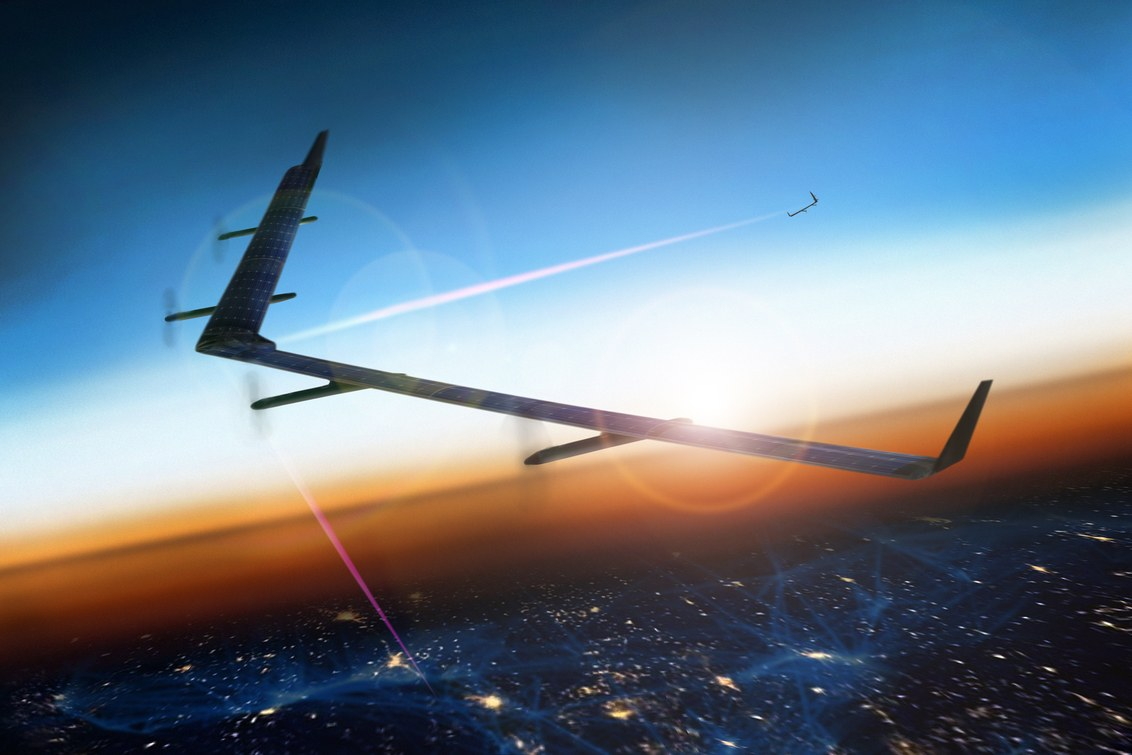
\includegraphics[height=4cm]{aquila.jpg}
    \pause
\Put(-150,90){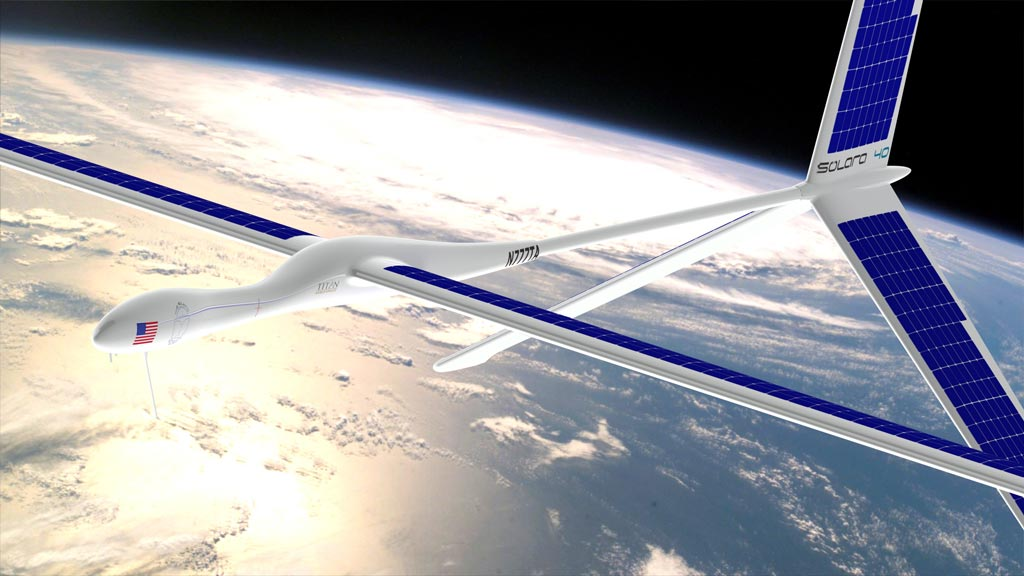
\includegraphics[height=4cm]{titan.jpg}}
    \pause
\Put(-130,80){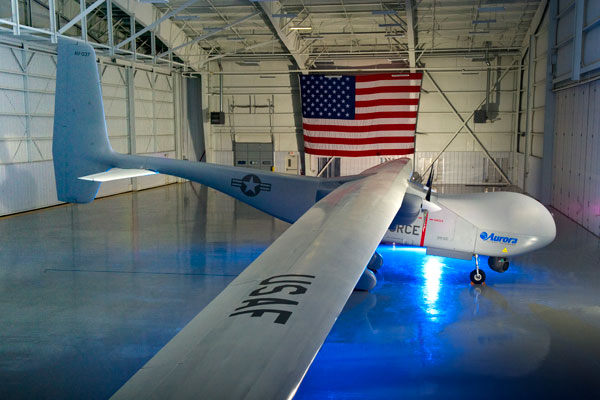
\includegraphics[height=4cm]{orion.jpg}}
    \pause
\Put(-100,70){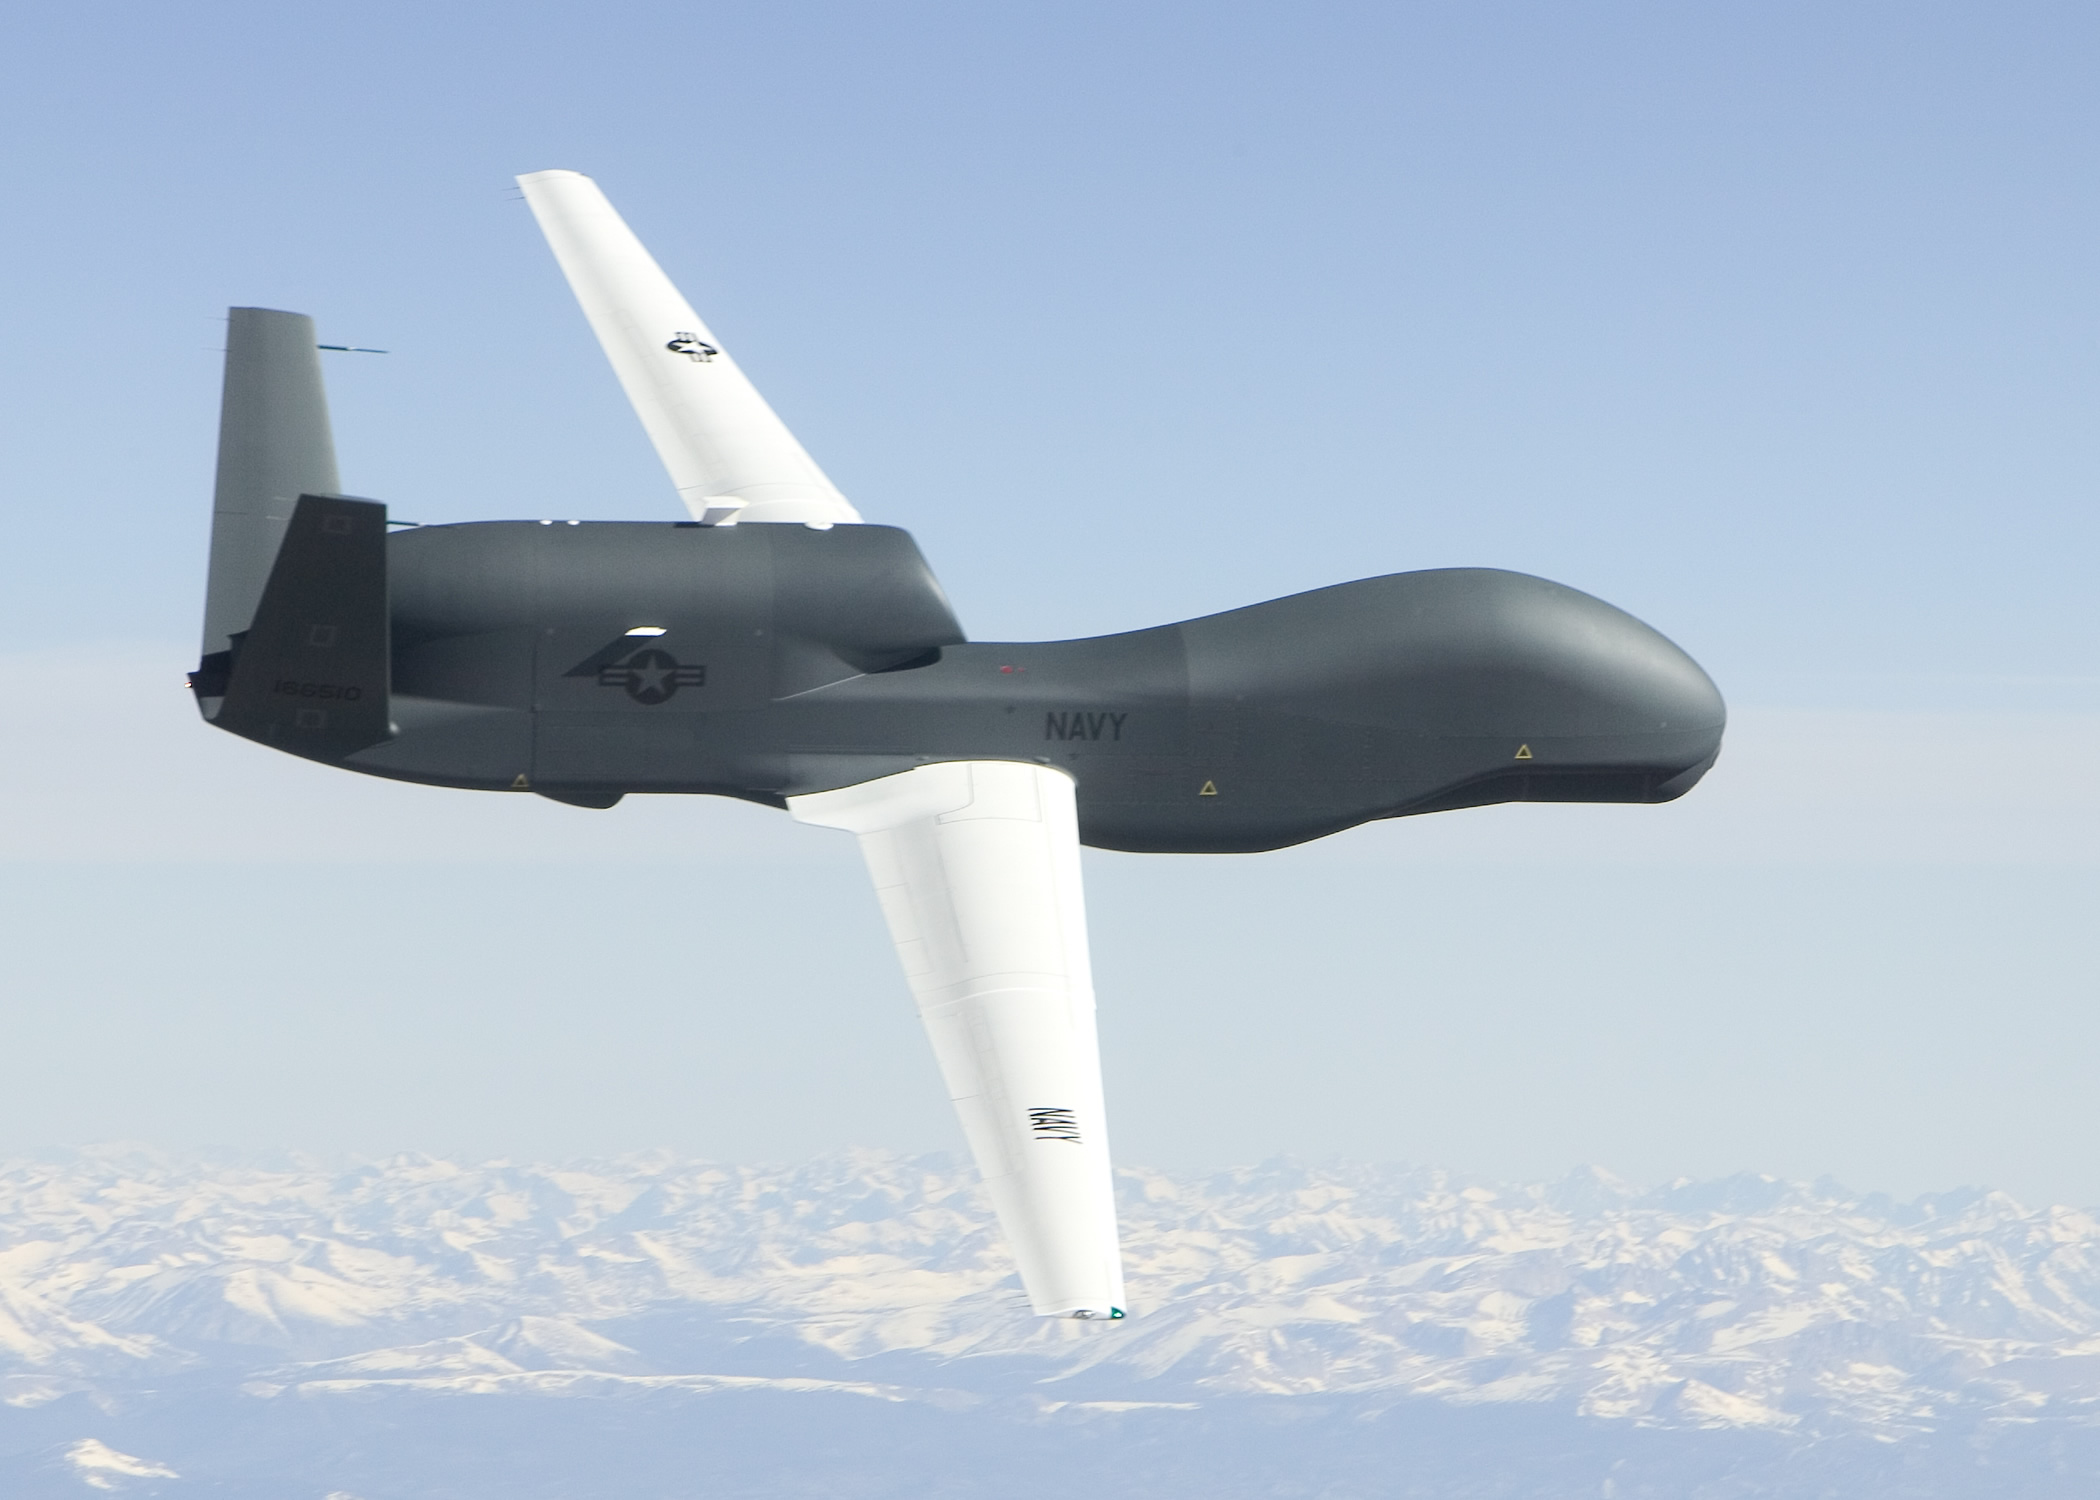
\includegraphics[height=4cm]{globalhawk.jpg}}
    \pause
\Put(-80,60){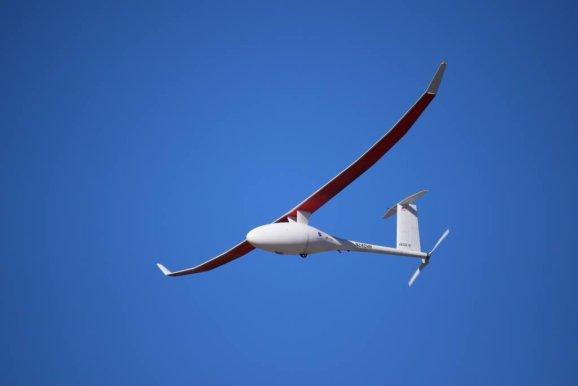
\includegraphics[height=4cm]{vanilla.jpg}}
    \pause
\Put(-60,60){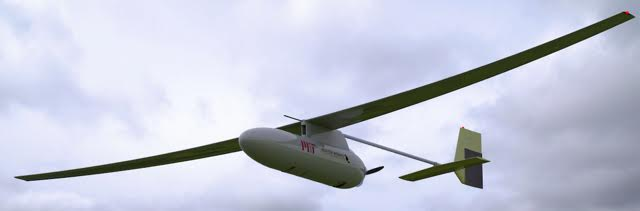
\includegraphics[height=3cm]{jho.jpeg}}

\end{frame}
 
\begin{frame}
    \frametitle{Limitations on Endurance}

    \begin{itemize}
        \item Gas: fuel 
        \item Solar-electric: winter solstice \\~\\
    \end{itemize}

    
    At 30$^{\circ}$ latitude:
    \begin{columns}
        \column{0.5\textwidth}
        \includegraphics[width=1.0\textwidth]{windvsmonth.pdf}
        
        \column{0.5\textwidth}
        \includegraphics[width=1.0\textwidth]{eirrvsmonth.pdf}
    \end{columns}

\end{frame}

\begin{frame}
    \frametitle{Latitude Requirement}

    \begin{center}
        (Example: operate between $\pm30^{\circ}$ latitude)
        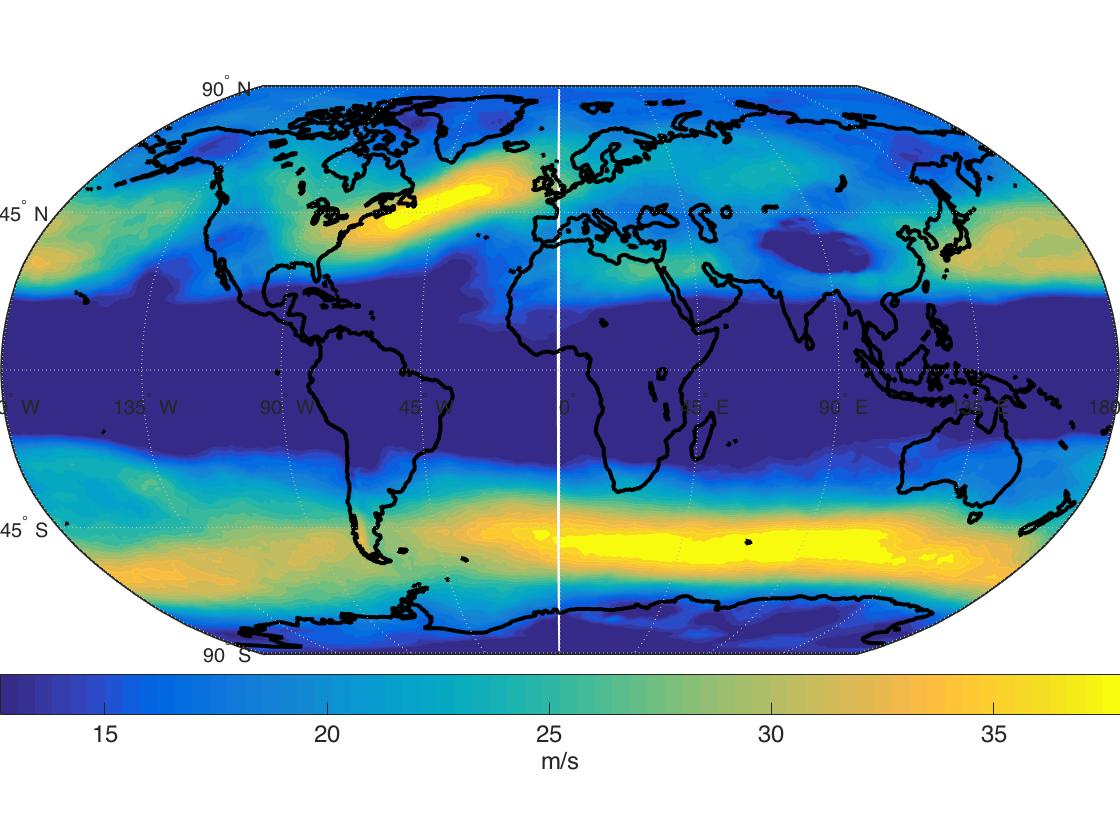
\includegraphics[width=0.8\textwidth]{worldwinds.jpg} \\
        \scriptsize
        95th Percentile Winds in 2015 at 15,000 ft
    \end{center}

\end{frame}

\begin{frame}
    \frametitle{Wind Speed by Latitude}

    \begin{center}
    \includegraphics[width=0.7\textwidth]{latvswind.pdf} \\
    \scriptsize
    80th, 90th, 95th Percentile Winds
    \end{center}

\end{frame}

\begin{frame}
    \frametitle{Operating Altitude}
    
    \begin{columns}
        \column{0.45\textwidth}
        \begin{itemize}
            \item Gas: determined by payload
                \begin{itemize}
                    \item (5,000 - 25,000 ft)
                    \end{itemize}
            \item Solar-electric: optimized 
                \begin{itemize}
                    \item (55,000 - 70,000 ft)
                    \end{itemize}
                \end{itemize}
        
        \column{0.55\textwidth}
        \includegraphics[width=1.0\textwidth]{altvswind.pdf}
    \end{columns}

\end{frame}

\begin{frame}
    \frametitle{Percentile Wind Speed}
    
    \begin{columns}
        \column{0.5\textwidth}
        \includegraphics[width=1.0\textwidth]{Boston_dec_2015.pdf}
        
        \column{0.5\textwidth}
        \includegraphics[width=1.0\textwidth]{Boston_dec_2015auto.pdf}
    \end{columns}

    \begin{center}
    Wind speeds in Boston, December 2015 at 60,000 ft. 
    \end{center}
    
\end{frame}

\begin{frame}
    \frametitle{Geometric Programming}
    \begin{itemize}
        \item Non-linear optimization \\~\\
        \item Can be solved extremely quickly \\~\\
        \item Guaranteed global optimum \\~\\
        \item No initial guess
        \end{itemize}
\end{frame}

\begin{frame}
    \frametitle{Example GP}

    \begin{columns}
        \column{0.5\textwidth}
        Form:
        \column{0.5\textwidth}
        Example:
    \end{columns}
    
    \begin{columns}
        \column{0.5\textwidth}
        \scriptsize
        \begin{align*}
            \text{minimize } &g_0(x) \\
            \text{subject to } &f_i(x) = 1, &i &= 1,\dots,m\\
                               &g_i(x) \leq 1, &i &= 1,\dots,n
        \end{align*}

        \begin{align*}
            f(\bold{x}) &= c x_1^{a_1} x_2^{a_2} \dotsm x_n^{a_n} , \\
            g(\bold{x}) &= \displaystyle\sum_{k=1}^K c_k x_1^{a_{1_k}} x_2^{a_{2_k}} \dotsm x_n^{a_{n_k}}.
        \end{align*}

        \column{0.5\textwidth}
        \scriptsize
        \begin{align*}
            \text{minimize } & x^{-1}y^{-1/2}z^{-1} + 2.3xz + 4xyz\\
            \text{subject to } &\frac{1}{3}x^{-2}y^{-2} + \frac{4}{3}y^{1/2}z^{-1} \leq 1\\
                              &x + 2y + 3z \leq 1
        \normalsize
        \end{align*}

    \end{columns}
\end{frame}

\begin{frame}
    \frametitle{Optimizing Wind Speed}

    \begin{align*}
        V &\geq V_{\text{wind}_i}, i = 20,\dots,\text{Lat. Req.} \\
        V_{\text{wind}} &= f(\rho, p_{\text{wind}})
    \end{align*}

    \begin{center}
    \includegraphics[width=0.6\textwidth]{windfitl35.pdf}
    \end{center}

\end{frame}

\begin{frame}
    \frametitle{Solar Energy}

    \scriptsize
    \[ \begin{array}{rrl}
        \text{Solar Energy} : & (E/S)_{\text{sun}}  &\geq (E/S)_{\text{day}} + \frac{E_{\text{batt}}}{\eta_{\text{charge}}\eta_{\text{solar}} S_{\text{solar}}} \\
        \text{Battery Energy} : &E_{\text{batt}} &\geq \frac{P_{\text{oper}}t_{\text{night}}}{\eta_{\text{discharge}}} + (E/S)_{\text{twilight}} \eta_{\text{solar}} S_{\text{solar}} \\
        \text{Minimum operational solar power} : & (P/S)_{\text{min}} &= \frac{P_{\text{oper}}}{\eta_{\text{solar}} S_{\text{solar}}} 
    \end{array} \]

    \begin{center}
    \includegraphics[width=0.7\textwidth]{lat30.pdf}
    \end{center}
\end{frame}

\begin{frame}
    \frametitle{Gas Endurance}

    \[ \text{Breguet Endurance}: t = \frac{W_{\text{ave}}}{P_{\text{shaft}}\text{BSFC}g} \ln{\left( \frac{W_{\text{initial}}}{W_{\text{final}}}\right)} \]
        
    \begin{center}
    \includegraphics[width=0.7\textwidth]{powertobsfcfit.pdf}
    \end{center}

\end{frame}
        
\begin{frame}
    \frametitle{Engine Sizing}

    \scriptsize
    \[ \begin{array}{rrl}
            \text{Climb Rate}: & \dot{h} &\geq 100 \text{ [ft/min]} \\
            \text{Lapse Rate Definition}: &L_{\text{eng}}(h) &\equiv \frac{P_{\text{max}}}{P_{\text{SL-max}}} \\
            \text{Approxmiate Lapse Rate Equation}: & L_{\text{eng}}(h) &= 1 - \frac{0.035}{1000 \text{ [ft]}} h
    \end{array} \]

    \begin{center}
    \includegraphics[width=0.7\textwidth]{powervsweightfit.pdf}
    \end{center}

\end{frame}

\begin{frame}
    \frametitle{Aerodyanmics}

    \[ C_D \geq C_{d_0} + c_{d_p} + \frac{C_L^2}{\pi e A} \]

    \begin{center}
    aircraft drag $\geq$ non-wing drag + wing profile drag + induced drag
    \includegraphics[width=0.7\textwidth]{JH01polar.pdf} \\
    \scriptsize
    JHO airfoil profile drag
    \end{center}
    
\end{frame}

\begin{frame}
    \frametitle{Wing Loading Cases}
      
    \begin{columns}
        \column{0.5\textwidth}
        \begin{center}
        Standard g-loading ($N_{\text{max}}$ = 5) \\
        Sizes gas powered aircraft \\~\\
        \end{center}
        
        \column{0.5\textwidth}
        \begin{center}
        Gust Loading ($N_{\text{max}}$ = 2) \\
        Sizes solar-electric aircraft \\~\\
        \end{center}
    \end{columns}

    \begin{columns}
        \column{0.5\textwidth}
        \includegraphics[width=1.0\textwidth]{gbending.pdf}
        
        \column{0.5\textwidth}
        \includegraphics[width=1.0\textwidth]{gustloaddiagram.pdf}
    \end{columns}
\end{frame}

\begin{frame}
    \frametitle{Discretized Beam}

    \begin{align*}
        \mathcal{S}_{i+1} &\geq \mathcal{S}_i + \frac{q_{i+1} + q_i}{2} \Delta y \\
        \mathcal{M}_{i+1} &\geq \mathcal{M}_i + \frac{\mathcal{S}_{i+1} + \mathcal{S}_i}{2} \Delta y \\
        \Theta_{i} &\geq \Theta_{i+1} + \frac{1}{2} \left(\frac{\mathcal{M}_i}{EI_i} + \frac{\mathcal{M}_{i-1}}{EI_{i-1}} \right) \Delta y \\
        w_{i} &\geq w_{i+1} + \frac{1}{2} (\Theta_i + \Theta_{i-1}) \Delta y 
    \end{align*}
\end{frame}

\begin{frame}
    \frametitle{Cap Spar}

    \begin{center}
    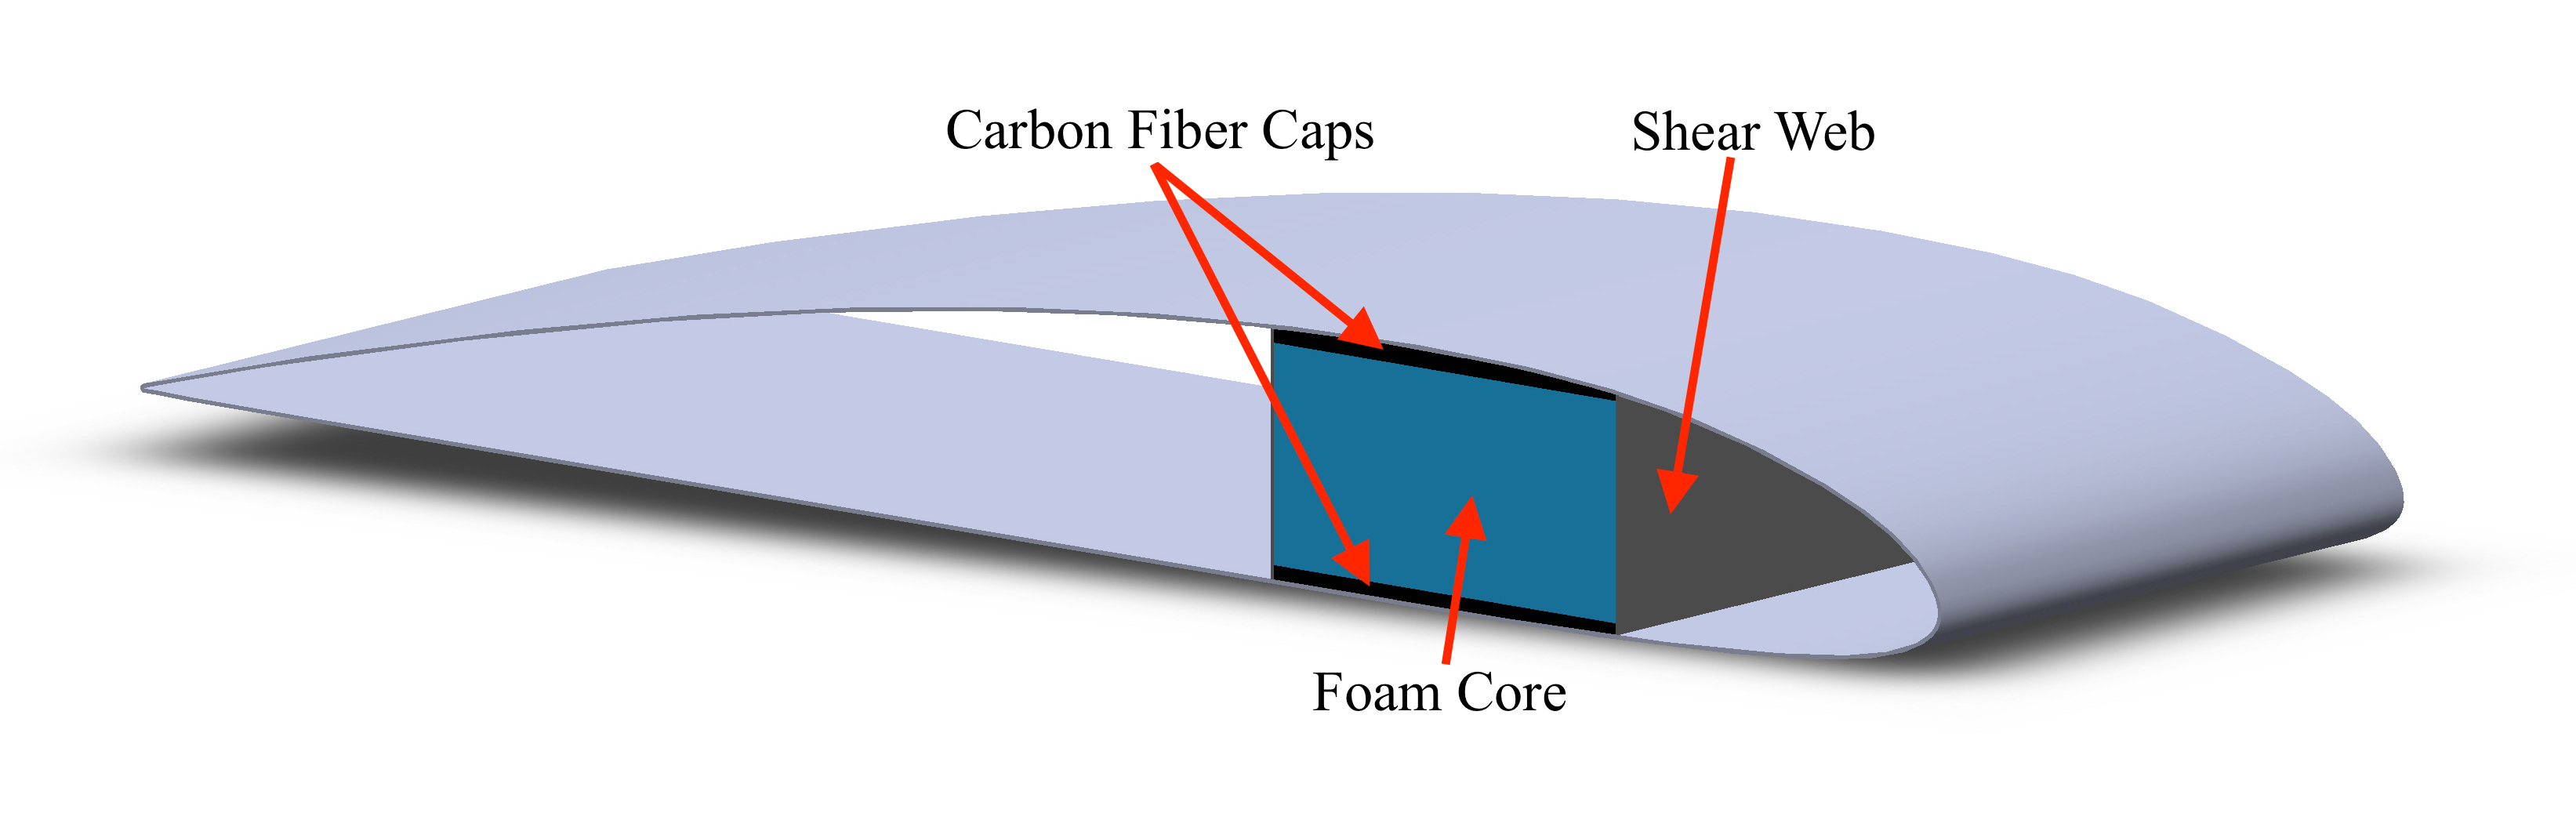
\includegraphics[width=0.8\textwidth]{capspar.jpg}
    \end{center}

    \begin{columns}
        \column{0.5\textwidth}
        \begin{center}
        Dimensional Constraints
        \end{center}
        \column{0.5\textwidth}
        \begin{center}
        Moment and Deflection Constraints
        \end{center}
    \end{columns}
    
    \begin{columns}
        \column{0.5\textwidth}
        \begin{align*}
            I_i &\leq 2w_{\text{cap}_i}t_{\text{cap}_i}\left(\frac{h_{\text{cap}_i}}{2}\right)^2 \\
            c(y)\tau_t &\geq h_{\text{cap}_i} + 2t_{\text{cap}_i} \\
            c(y)\tau_w &\geq w_{\text{cap}_i} 
        \end{align*}

        \column{0.5\textwidth}
        \begin{align*}
            \sigma_{\text{cfrp}} &\geq \mathcal{M}_i \frac{h_{\text{cap}_i}+t_{\text{cap}_i}}{I_i}\\
            w_n &\leq w_{\text{max}}
        \end{align*}
        
    \end{columns}

\end{frame}

\begin{frame}
    \frametitle{Configuration}

    \begin{center}
    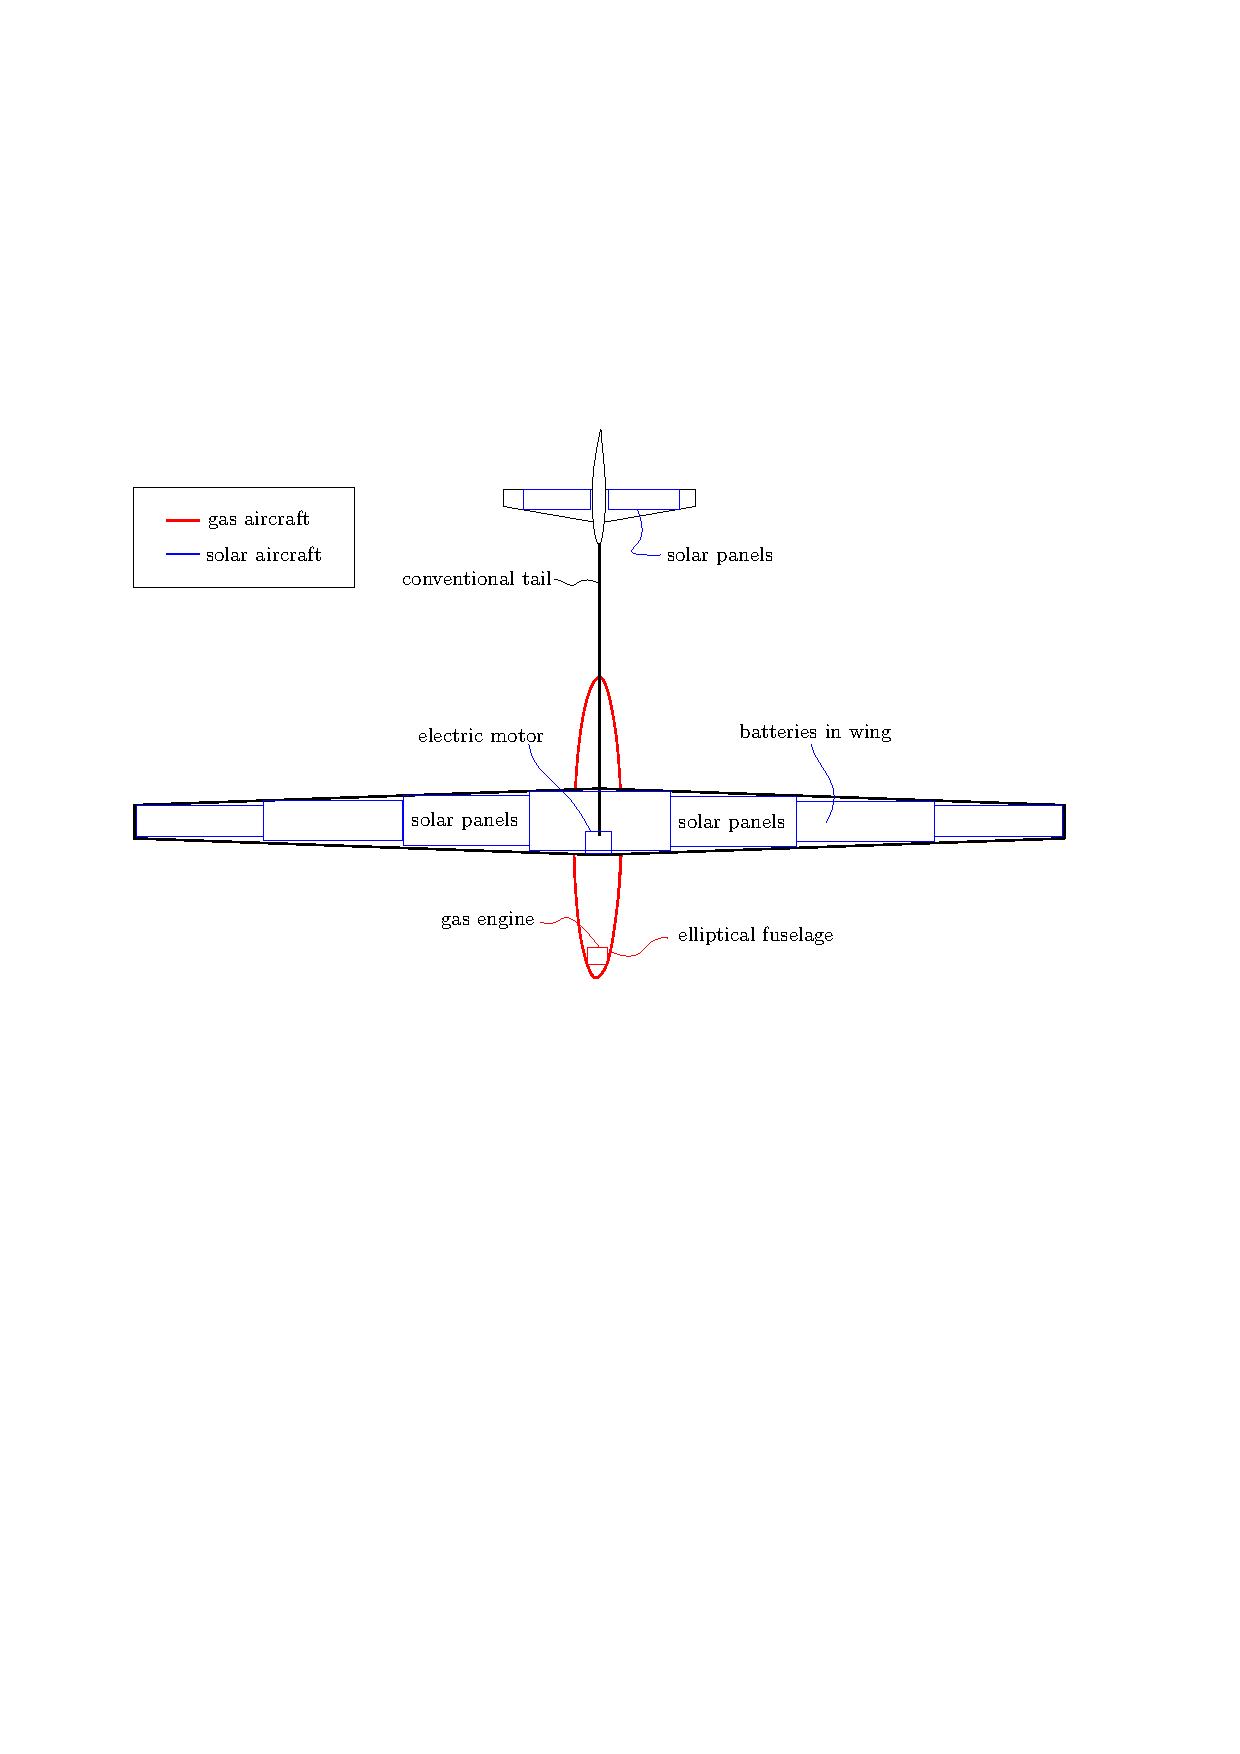
\includegraphics[width=1.0\textwidth]{simpleaircraft.pdf}
    \end{center}

\end{frame}

\begin{frame}
    \frametitle{Configuration}
    
    \begin{columns}
        \column{0.5\textwidth}
        \begin{center}
        Component Weight
        \end{center}
        \column{0.5\textwidth}
        \begin{center}
        Component Drag
        \end{center}
    \end{columns}

    \begin{columns}
        \column{0.5\textwidth}
        \scriptsize
        \begin{align*}
        W_{\text{skin}} &\geq 2 \rho_{A_{\text{cfrp}}} S g \\
        W_{\text{boom}} &\geq \pi \rho_{\text{cfrp}} t_0 d l_{\text{h}}g \left( 1 - \frac{1}{2} k\right) \\
        W_{\text{h}}/m_{\text{fac}} &\geq \rho_{\text{foam}} \frac{S_{\text{h}}^2}{b_{\text{h}}} \bar{A} + g\rho_{A_{\text{cfrp}}} S_{\text{h}} \\
        W_{\text{v}}/m_{\text{fac}} &\geq \rho_{\text{foam}} \frac{S_{\text{v}}^2}{b_{\text{v}}} \bar{A} + g\rho_{A_{\text{cfrp}}} S_{\text{v}} \\
            W_{\text{fuse}} &\geq S_{\text{fuse}} \rho_{A_{\text{cfrp}}} g
        \end{align*}
        \column{0.5\textwidth}
        \scriptsize
        \begin{align*}
        D_{\text{boom}} &\geq \frac{1}{2} C_f \rho V^2 l_{\text{h}}\pi d \\
        D_{\text{fuse}} &\geq C_f k_{\text{fuse}} \frac{1}{2} \rho V^2 S_{\text{fuse}} \\
        C_f &\geq \frac{0.455}{Re^{0.3}} \\
        D_{\text{h}} &\geq \frac{1}{2} c_{d_{\text{h}}} \rho V^2 S_{\text{h}} \\
        D_{\text{v}} &\geq \frac{1}{2} c_{d_{\text{v}}} \rho V^2 S_{\text{v}} 
        \end{align*}
    \end{columns}

\end{frame}

\begin{frame}
    \frametitle{Weight Breakdown}

    Gas Aircraft
    \begin{align*}
        \text{MTOW} &\geq W_{\text{structural}}  + W_{\text{payload}} + W_{\text{fuel}} + W_{\text{engine}} \\
        W_{\text{structural}} &\geq W_{\text{wing}} + W_{\text{boom}} + W_{\text{h}}+ W_{\text{v}} + W_{\text{fuse}}
    \end{align*}

    Solar-electric Aircraft
    \begin{align*}
        \text{MTOW} &\geq W_{\text{structural}} + W_{\text{payload}} + W_{\text{solar}} + W_{\text{batt}} + W_{\text{motor}} \\
        W_{\text{structural}} &\geq W_{\text{wing}} + W_{\text{boom}} + W_{\text{h}}+ W_{\text{v}} \\
        W_{\text{solar}} &\geq \rho_{\text{solar}} S_{\text{solar}} g \\
        W_{\text{batt}} &\geq \frac{E_{\text{batt}}}{h_{\text{batt}}} g \\
        E_{\text{batt}} &= 350 \text{ [Whr/kg]}
    \end{align*}

\end{frame}

\begin{frame}
    \frametitle{Weight vs Latitude}

    \begin{center}
    \includegraphics[width=0.7\textwidth]{mtowvslat.pdf} \\
    Minimize MTOW
    \end{center}

\end{frame}

\begin{frame}
    \frametitle{Solar Feasibility}

    \begin{center}
    \includegraphics[width=0.7\textwidth]{battsolarcontour.pdf} \\
    Minimizing battery specific energy for solar cell efficiency sweeps, 90th percentile wind speeds
    \end{center}

\end{frame}

\begin{frame}
    \frametitle{Gas Powered Endurance}

    \begin{center}
    \includegraphics[width=0.7\textwidth]{mtowvsendurance.pdf} \\
    Minimizing MTOW
    \end{center}

\end{frame}

\begin{frame}
    \frametitle{Changing Objectives on Solar Aircraft}

    \begin{columns}
        \column{0.5\textwidth}
        \includegraphics[width=1.0\textwidth]{solarobjcomp.pdf}
        
        \column{0.5\textwidth}
        \includegraphics[width=1.0\textwidth]{solarobjcomp2.pdf}
    \end{columns}
    \begin{center}
        90th percentile wind speeds
    \end{center}

\end{frame}

\begin{frame}
    \frametitle{Changing Structural Models on Solar Aircraft}

    \[ W_{\text{structural}} \geq \text{MTOW} f_{\text{structural}} \]

    \begin{center}
    \includegraphics[width=0.7\textwidth]{windaltoper.pdf} \\
    Minimizing MTOW, 90th percentile wind speeds
    \end{center}

\end{frame}

\begin{frame}
    \frametitle{With and Without Wind Speed Constraint}

    \begin{center}
    \includegraphics[width=0.7\textwidth]{polarmission.pdf} \\
    Minimizing MTOW, 90th percentile wind speeds
    \end{center}

\end{frame}

\begin{frame}
    \frametitle{Solar-electric Aircraft Sensitivities}

    \tiny
    \begin{longtable}{lccccccccccccc}
        \toprule
        \toprule
        \multirow{2}{*}{Variable}& 25th Latitude & 30th Latitude & 25th Latitude & 30th Latitude \\
                                 & 85th Percentile Winds & 85th Percentile Winds & 90th Percentile Winds & 90th Percentile Winds \\
        \midrule
        $\eta_{\text{prop}}$ &-3.58 & -3.89 & -8.62 & -13.6\\
        $\eta_{\text{discharge}}$ &-2.8 & -3.04 & -6.61 & -10.3\\
        $t_{\text{night}}$ &2.8 & 3.04 & 6.61 & 10.3\\
        $h_{\text{batt}}$ &-2.27 & -2.45 & -4.74 & -7.23\\
        $\eta_{\text{solar}}$ &-1.29 & -1.43 & -3.85 & -6.28\\
        $(E/S)_{\text{sun}}$ &-1.15 & -1.28 & -3.58 & -5.87\\
        $p_{\text{wind}}$ &1.12 & 1.86 & 3.05 & 7.59\\
        $W_{\text{pay}}$ &0.738 & 0.73 & 0.816 & 0.967\\
        $\eta_{\text{charge}}$ &-0.707 & -0.784 & -2.25 & -3.68\\
        $\rho_{\text{solar}}$ &0.261 & 0.281 & 0.614 & 0.938\\
        \bottomrule
    \end{longtable}

\end{frame}

\begin{frame}
    \frametitle{Gas Aircraft Sensitivities}

    \scriptsize
    \begin{longtable}{lccccccccccccc}
        \toprule
        \toprule
        Variable & 5 Day Endurance & 7 Day Endurance & 9 Day Endurance\\
        \midrule
        $V_{\text{wind}}$ &1.76 & 2.87 & 6.93\\
        $\eta_{\text{prop}}$ &-1.63 & -2.7 & -7.41\\
        $\text{BSFC}_{100\%}$ &1.55 & 2.6 & 7.12\\
            $t_{\text{endurance}}$ &1.46 & 2.48 & 6.91\\
        $W_{\text{pay}}$ &0.251 & 0.188 & 0.117\\
        $N_{\text{max}}$ &0.16 & 0.323 & 1.26\\
        \bottomrule
        \end{longtable}
    
\end{frame}

\begin{frame}
    \frametitle{Contributions}

    \begin{itemize}
        \item Comparison of long-endurance UAV archictures \\~\\
        \item Solar-electric and gas powered sizing analysis \\~\\
        \item Defined solar-electric operational feasilibity \\~\\
        \end{itemize}


\end{frame}

\end{document}
